\documentclass[12pt]{article}
\usepackage[T1]{fontenc}
\usepackage[T1]{polski}
\usepackage[utf8]{inputenc}
\usepackage{color}
\usepackage{graphicx}
\usepackage{blindtext}
\usepackage{scrextend}
\newcommand{\BibTeX}{{\sc Bib}\TeX} 
\usepackage{graphicx}
\usepackage{amsfonts}

\setlength{\textheight}{21cm}

\title{{\bf Zadanie nr 3 - Splot, filtracja i korelacja sygnałów}\linebreak
Cyfrowe Przetwarzanie Sygnałów}
\author{Aneta Wiśniewska, 204029 \and Hanna Paluszkiewicz, 203962}
\date{14.05.2018}

\begin{document}
\clearpage\maketitle
\thispagestyle{empty}
\newpage
\setcounter{page}{1}
\section{Cel zadania}

Celem ćwiczenia jest zapoznanie się w praktyce z procesami splotu, filtracji i korelacji sygnałów. Aby to osiągnąć, trzeba napisać aplikację umożliwiającą przetwarzanie analgowo-cyfrowe z uwzględnieniem operacji próbkowania i kwantyzacji oraz konwersji odwrotnej, tj. cyfrowo-analogowej (w naszym przypadku tylko interpolacja i ekstrapolacja).

\section{Wstęp teoretyczny}

\subsection{Teoria}


\addtokomafont{labelinglabel}{\sffamily}

\begin{labeling}{alligator}
\item [Splot] to jedno z najważniejszych działań podczas filtracji sygnałów dyskretnych. Jest operacją przetwarzania dwóch sygnałów, w wyniku której otrzymujemy pojedyńczy sygnał dyskretny.  W ogólnym przypadku splot jest zdefiniowany wzorem:
\begin{figure}[h!]
 \centering
 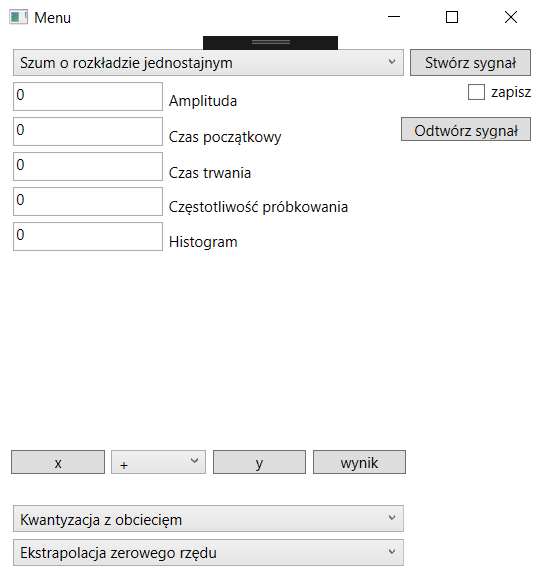
\includegraphics[width=9.3cm]{ui1.PNG}
 \vspace{-0.3cm}
 \caption{Widok główny aplikacji}
 \label{Widok_aplikacjis}
\end{figure}
W praktyce stosuje się sygnały o skończonych ilosciach próbek rozmieszczonych równomiernie w dowolnych miejscach osi czasu. Zwykle przyjmuje się konwencję indeksacyjną, gdzie oba sygnały zaczynają się  na osi czasu od próbki zero. Poza granicami przedziału oba sygnały są zerowe. 
\\Wzór dla tej konwencji przyjmuje postać: 
\begin{figure}[h!]
 \centering
 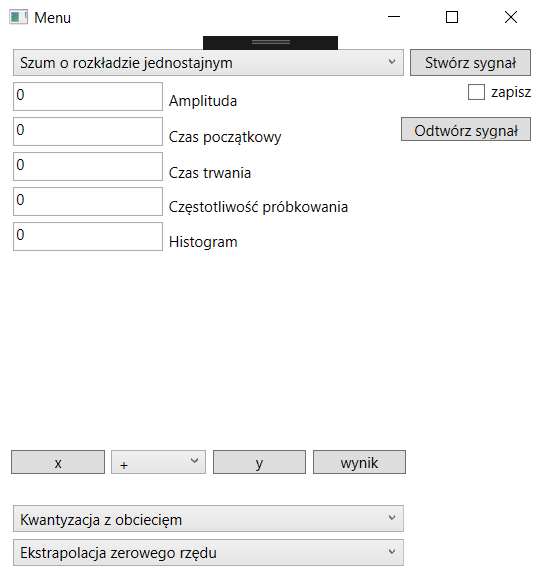
\includegraphics[width=9.3cm]{ui1.PNG}
 \vspace{-0.3cm}
 \caption{Widok główny aplikacji}
 \label{Widok_aplikacjis}
\end{figure}

\item [Filtracja sygnałów]  - należy do podstawowych operacji CPS. W ramach filtracji widmo sygnału ulega modyfikacji. Zostały odfiltrowane składowe częci sygnału o częstotliwosciach należących do pasma zaporowego. Reszta widma leżąca w pamie przepustowym, nie uległa zmianie lub podlega niewielkiemu tłumieniu. 
\\Filtry ze względu na umiejscowienie pasma przepustowego i zaporowego dzielimy na:
\subitem [Filtry dolnoprzepustowe] - dsfhis 
\subitem [filtry górnoprzepustowe]
\subitem [filtry pasmowe]

\item [Korelacja] - jest ważną częscią przetwarzania sygnałów. Jest stosowana, gdy trzeba porównać sygnał z innym, zwłaszcza z przesuniętą na osi czasu swoją kopią.
Polega na przetwarzaniu dwóch sygnałów dyskretnych, w czego wyniku otrzymujemy pojedynczy sygnał dyskretny.
\\Korelacja w ogólnym przypadku jest opisywana wzorem"
\begin{figure}[h!]
 \centering
 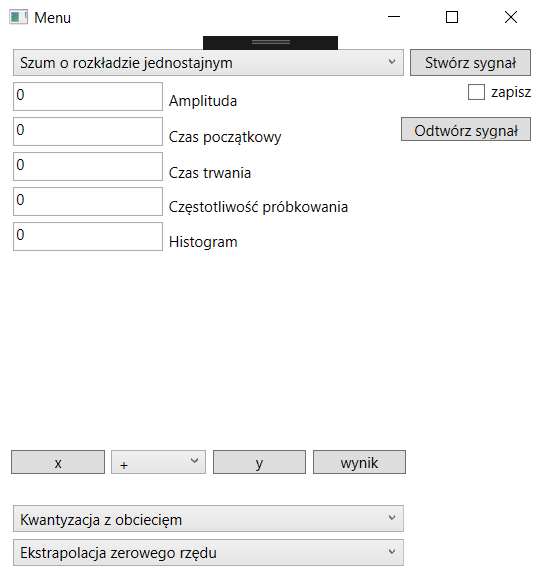
\includegraphics[width=9.3cm]{ui1.PNG}
 \vspace{-0.3cm}
 \caption{Widok główny aplikacji}
 \label{Widok_aplikacjis}
\end{figure}
\\Podobnie jak w operacji splotu w praktyce............................................................................................................
\\Opisanym wzorem:
\begin{figure}[h!]
 \centering
 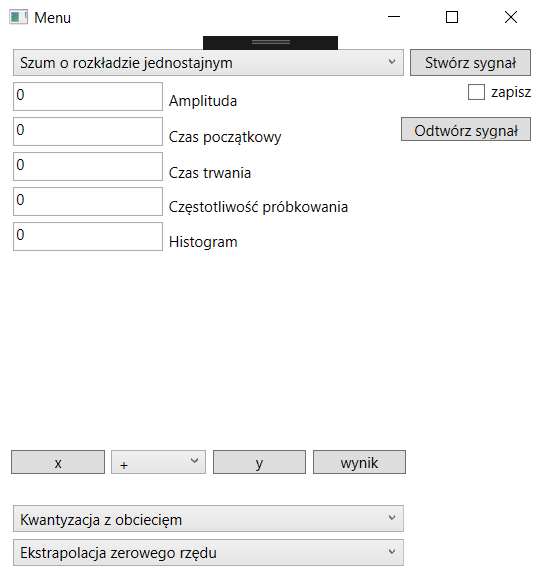
\includegraphics[width=9.3cm]{ui1.PNG}
 \vspace{-0.3cm}
 \caption{Widok główny aplikacji}
 \label{Widok_aplikacjis}
\end{figure}

\end{labeling}


\subsection{Instrukcja obsługi aplikacji}
Aplikacja do generacji szumów zawiera interfejs graficzny, który służy do obsługi przez użytkownika. Wygląd został przedstawiony na poniższym rysunku.
\newpage
\begin{figure}[h!]
 \centering
 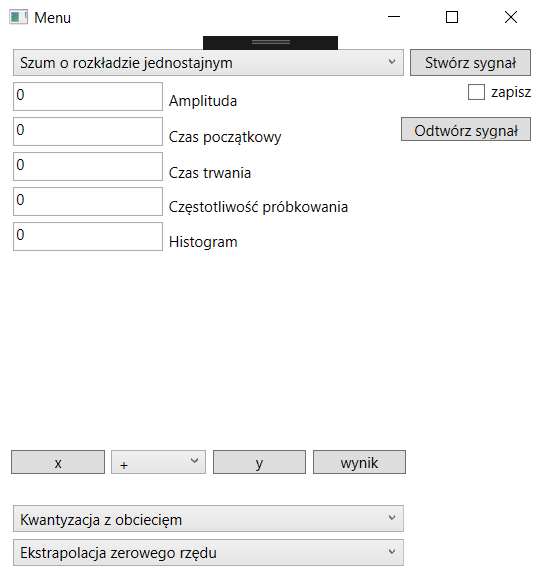
\includegraphics[width=9.3cm]{ui1.PNG}
 \vspace{-0.3cm}
 \caption{Widok główny aplikacji}
 \label{Widok_aplikacjis}
\end{figure}

Na górze okienka znajduje się wysuwana lista możliwych do generacji sygnałów. Obok znajduje się chceckbox, po zaznaczeniu którego sygnał zostanie zapisany do pliku.
Niżej jest przycisk do generacji sygnałów oraz lista parametrów wykresu. Tutaj wpisuje się dane wpływające na sygnał.
Pola umożliwiają ustawienie charakterystycznych parametrów sygnału. Na ich podstawie program wylicza wartości amplitudy sygnału w określonym czasie oraz wyświetla graficzną reprezentację sygnału w postaci wykresu funkcji amplitudy od czasu i histogramu.\\

Na dole okienka znajdują się przyciski: do odtwarzania sygnału z pliku, oraz do operacji na dwóch sygnałach. Po kliknięciu w x i y wybieramy odpowiednio pierwszy i dugi składnik działania. Między nimi można wybrać jedno z czterech działań.  Po wcisnięciu przycisku "wynik" program liczy wynik działania i wywietla jego graficzną reprezentację. 

\subsubsection{Generowanie sygnału}
Aby wygenerować sygnał użytkownik musi kliknąć w generuj sygnał.
\\Po wygenerowaniu sygnału pojawiają się dwa dodatkowe okienka aplikacji.
\begin{figure}[h!]
 \centering
 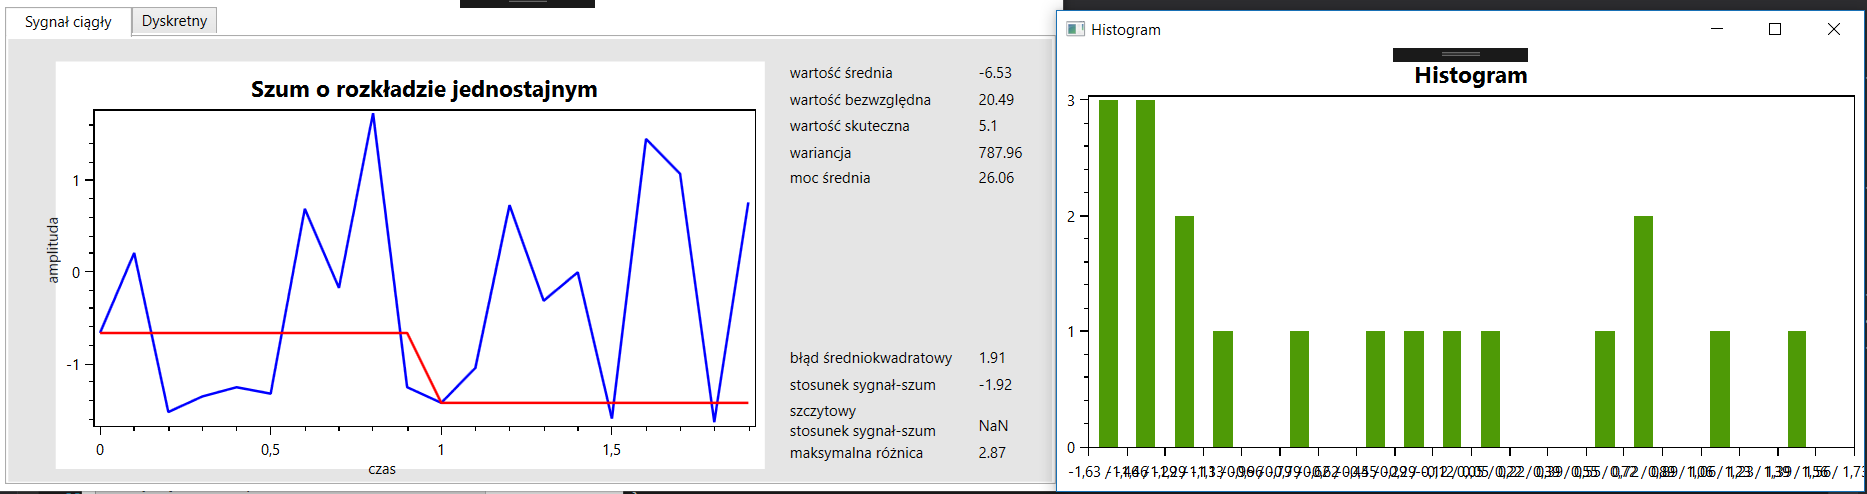
\includegraphics[width=15.3cm]{okienka.PNG}
 \vspace{-0.3cm}
 \caption{Okna po generacji sygnału}
 \label{Widok_aplikacjis}
\end{figure}
\\Jedno wyświetla histogram sygnału
\\Drugie przedstawia wykres funkcji amplitudy od czasu oraz obliczone wartości: wartość średnią, wartość średnią bezwzględną, wartość skuteczną, wariancję oraz moc średnią.

\subsubsection{Odczyt sygnału z pliku}
Oprócz generacji i zapisu do pliku, program umożliwia odczyt z pliku sygnału będącego wynikiem dyskretyzacji (bez kwantyzacji) wygenerowanego
sygnału ciągłego oraz sygnału będącego wynikiem operacji na dwóch sygnałach dyskretnych.
\\Tak jak w przypadku generacji, sygnał jest  reprezentowany graficznie w postaci histogramu i wykresu funkcji.

\subsection{Opis metod}
Opisy wszystkich metod zastosowanych do implementacji sygnałów, zostały zapisane w poszczególnych eksperymentach. 
\\ Próbkowanie pozwala na zmianę analogowego sygnału wejsciowego w sygnał dyskretny:
\begin{figure}[h!]
 \centering
 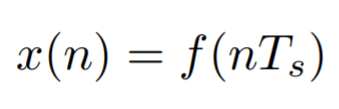
\includegraphics[width=3.3cm]{WzorProbkowanie.PNG}
 \vspace{-0.3cm}
 \label{Wykres}
\end{figure}
reprezentowany jako ciąg próbek rozmieszczonych równomiernie w czasie w odstępach Ts. Twierdzenie o próbkowaniu okresla możliwosć odtworzenia oryginalnego sygnału analogowego przy założeniu, że częstotliwosć próbkowania
\begin{figure}[h!]
 \centering
 \includegraphics[width=2.3cm]{cz.PNG}
 \vspace{-0.3cm}
 \label{cz}
\end{figure}
jest przynajmniej dwukrotnie wyższa niż najwyższa częstotliwosć  jakiejkolwiek składowej sygnału.
\subsection{Opis implementacji}
Aplikacja została napisana w wysokopoziomowym języku programowania - C\#. Do rysowania wykresów została wykorzystana zewnątrzna biblioteka OxyPlot. Program został napisany przy pomocy metodyki obiektowej i stosuje metody numeryczne.

\section{Eksperymenty i wyniki}

Poniżej znajdują się wszystkie przeprowadzone eksperymenty - możliwe do uzyskania w aplikacji sygnaly i wyniki. 

%%%%%%%%%%%%%%%%%%%%%%%%%%%%%%%%%%%%%%%%%%%%%%%%%%%%%%%%%%%%%%%%%%%%%%%%%%%%%%%%%%%%%%%%%%%%%%%%%%%%%%%%%%%%%%%%%
% PODROZDZIA PT. EKSPERYMENT NR 1 
%%%%%%%%%%%%%%%%%%%%%%%%%%%%%%%%%%%%%%%%%%%%%%%%%%%%%%%%%%%%%%%%%%%%%%%%%%%%%%%%%%%%%%%%%%%%%%%%%%%%%%%%%%%%%%%%%

\subsection{Eksperyment nr 1}

Eksperyment nr 1 -  Splot\\


\subsubsection{Założenia}
Do eksperymentu generujemy sygnał sinusoidalny o podanych niżej parametrach. Wejciowy sygnał analogowy zostanie zamieniony na sygnał dyskretny.
Sygnał opisuje wzór:

\begin{figure}[h!]
 \centering
 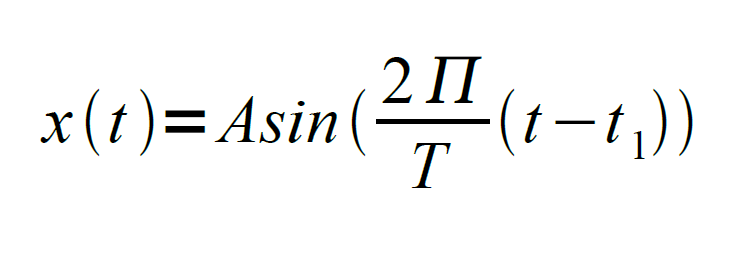
\includegraphics[width=4.3cm]{SinWzor.PNG}
 \vspace{-0.3cm}
 \label{gw}
\end{figure}
Parametry: A, T, t1, d.

W tym eksperymencie odtworzenie sygnału odbywa się porzez interpolację pierwszego rzędu, a dysktretyzacja przez kwantyzację z odcięciem. W tej metodzie wartosci sygnału pomiędzy sąsiednimi próbkami są interpolowwane za pomocą odcinków prostej.

\subsubsection{Przebieg}
Do generacji synału zostały podane parametry:
\addtokomafont{labelinglabel}{\sffamily}

\begin{labeling}{szj}
\item [Amplituda (A):] 2
\item [Czas trwania (t1):] 2 s
\item [Częstotliwość próbkowania (d): ] 10 Hz
\item [Okres podstawowy :] 1 s
\end{labeling}

\subsubsection{Rezultat}

Rezultaty przedstawiają zamieszczone poniżej zrzuty ekranu z programu. Wartości liczbowe oraz wykres funkcji amplitudy od czasu przedstawia \ref{Wykres dla wynikw eksperymentu pierwszego}.
\begin{figure}[h!]
 \centering
 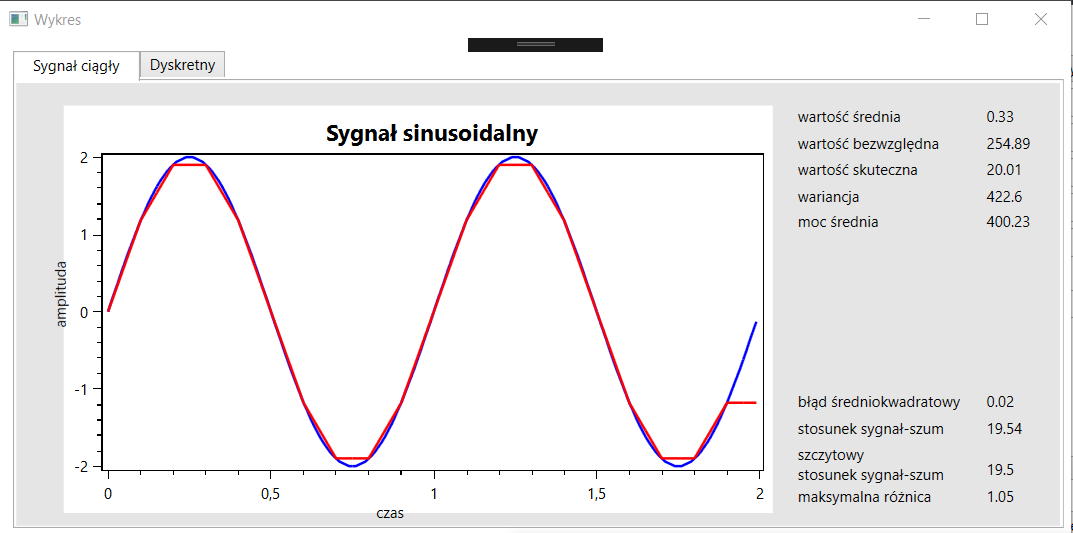
\includegraphics[width=12.3cm]{SinKwantObcIntA2T2f10H2t1C.PNG}
 \vspace{-0.3cm}
 \caption{Wykres sygnału sinusoidalnego ciągły: kwantyzacja z obcięciem, interpolacja pierwszego rzędu}
 \label{Wykres dla wynikw eksperymentu pierwszego}
\end{figure}

\newpage
Rys. \ref{Wykres dla wynikw eksperymentu pierwszego h} przedstawia histogram sygnału z opisanymi powyżej parametrami. 

\begin{figure}[h!]
 \centering
 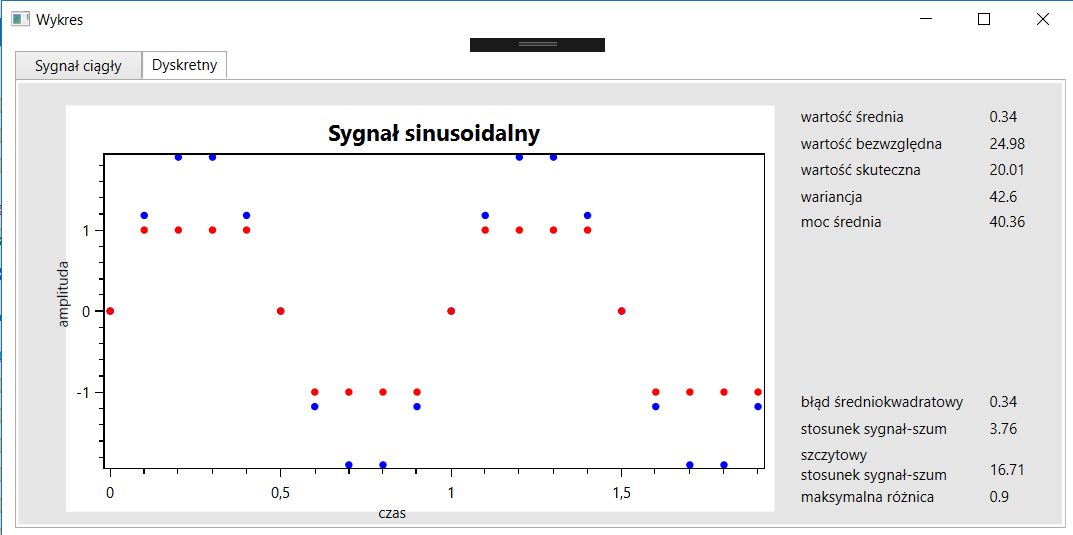
\includegraphics[width=12.3cm]{SinKwantObcIntA2T2f10H2t1D.PNG}
 \vspace{-0.3cm}
 \caption{Wykres sygnału sinusoidalnego dyskretny: kwantyzacja z obcięciem, interpolacja pierwszego rzędu}
 \label{Wykres dla wynikw eksperymentu pierwszego h}
\end{figure}

%%%%%%%%%%%%%%%%%%%%%%%%%%%%%%%%%%%%%%%%%%%%%%%%%%%%%%%%%%%%%%%%%%%%%%%%%%%%%%%%%%%%%%%%%%%%%%%%%%%%%%%%%%%%%%%%%
% PODROZDZIA PT. EKSPERYMENT NR2 
%%%%%%%%%%%%%%%%%%%%%%%%%%%%%%%%%%%%%%%%%%%%%%%%%%%%%%%%%%%%%%%%%%%%%%%%%%%%%%%%%%%%%%%%%%%%%%%%%%%%%%%%%%%%%%%%%

\subsection{Eksperyment nr 2}

Eksperyment nr 2  - Filtracja
\subsubsection{Założenia}
Sygnał opisuje wzór:

\begin{figure}[h!]
 \centering
 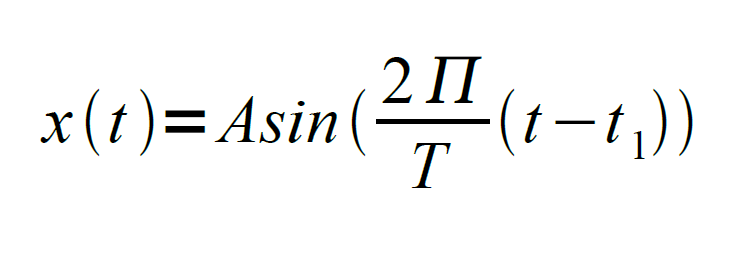
\includegraphics[width=4.3cm]{SinWzor.PNG}
 \vspace{-0.3cm}
 \label{gw}
\end{figure}
Parametry: A, T, t1, d.

\subsubsection{Przebieg}
Do generacji synału zostały podane parametry:
\addtokomafont{labelinglabel}{\sffamily}

\begin{labeling}{szj}
\item [Amplituda (A):] 2
\item [Czas trwania (t1):] 2 s
\item [Częstotliwość próbkowania (d): ] 10 Hz
\item [Okres podstawowy :] 1 s
\end{labeling}
\subsubsection{Rezultat}

Rezultaty przedstawiają zamieszczone poniżej zrzuty ekranu z programu. Wartości liczbowe oraz wykres funkcji amplitudy od czasu przedstawia \ref{Histogram dla wyników eksperymentu drugiego}.
\begin{figure}[h!]
 \centering
 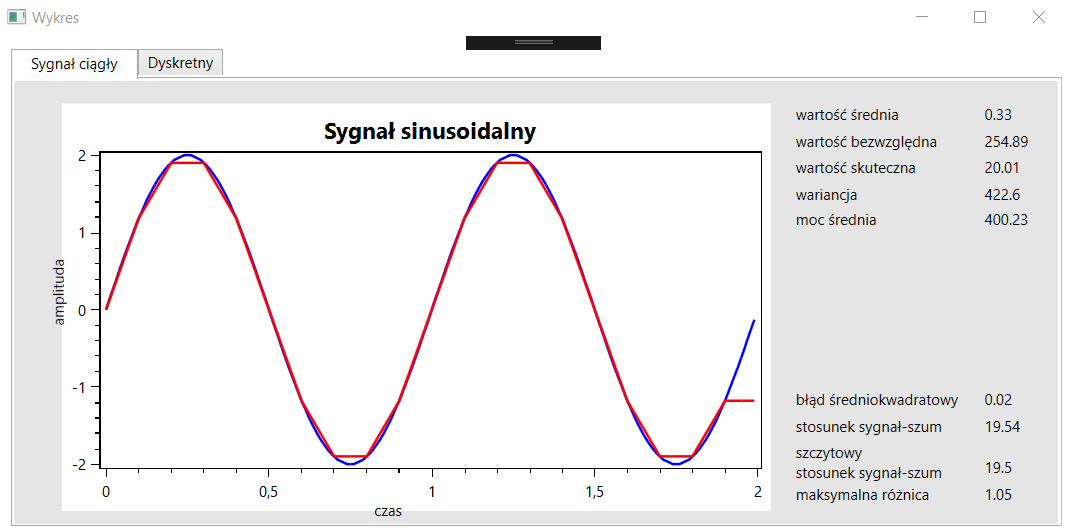
\includegraphics[width=12.3cm]{SinKwantZaokrIntA2T2f10H2t1C.PNG}
 \vspace{-0.3cm}
 \caption{Wykres sygnału sinusoidalnego ciągły: kwantyzacja z zaokrągleniem, interpolacja pierwszego rzędu}
 \label{Wykres dla wyników eksperymentu drugiego}
\end{figure}
\newpage
Rys. \ref{Wykres dla wynikw eksperymentu pierwszego h} przedstawia histogram sygnału z opisanymi powyżej parametrami. 
\begin{figure}[h!]
 \centering
 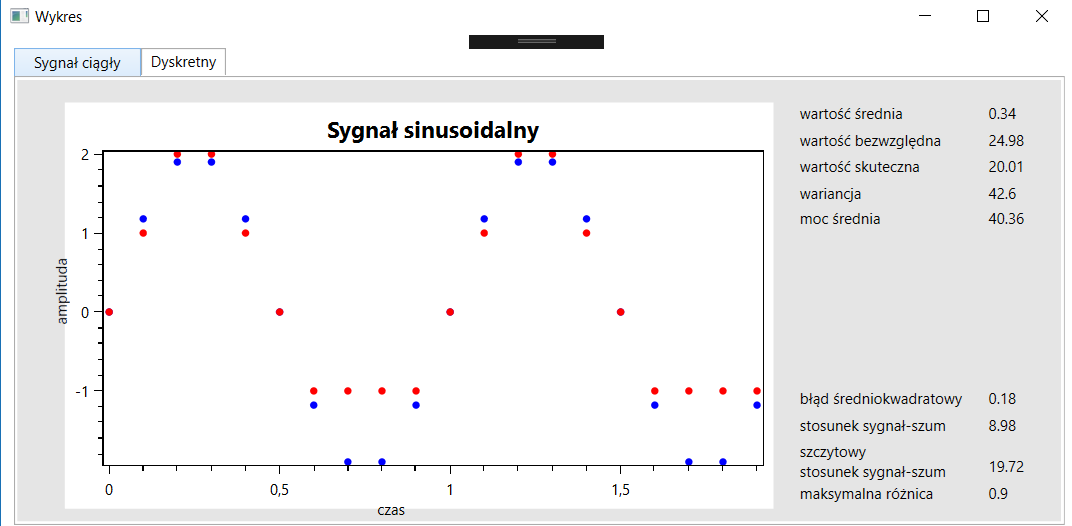
\includegraphics[width=12.3cm]{SinKwantZaokrIntA2T2f10H2t1D.PNG}
 \vspace{-0.3cm}
 \caption{Wykres sygnału sinusoidalnego dyskretny: kwantyzacja z zaokrągleniem, interpolacja pierwszego rzędu}
 \label{Histogram dla wyników eksperymentu drugiego}
\end{figure}

%%%%%%%%%%%%%%%%%%%%%%%%%%%%%%%%%%%%%%%%%%%%%%%%%%%%%%%%%%%%%%%%%%%%%%%%%%%%%%%%%%%%%%%%%%%%%%%%%%%%%%%%%%%%%%%%%
% PODROZDZIA PT. EKSPERYMENT NR 3 
%%%%%%%%%%%%%%%%%%%%%%%%%%%%%%%%%%%%%%%%%%%%%%%%%%%%%%%%%%%%%%%%%%%%%%%%%%%%%%%%%%%%%%%%%%%%%%%%%%%%%%%%%%%%%%%%%

\subsection{Eksperyment nr 3}

Eksperyment nr 3  Korelacja

\subsubsection{Teoria}
Ekstrapolacja zerowego rzędu jest najprostszą metodą rekonstrukcji sygnału. W  niej wartosć próbki jest pamiętana i definiuje stałą wartosć sygnału wyjsciowego aż do następnej próbki. Do tej metody potrzeba dużo wiekszej częstotliwosci próbkowania niż wynikałoby z "Twierdzenia o próbkowaniu". 

\subsubsection{Założenia}
Ekstrapolacja zerowego rzędu
Sygnał opisuje wzór:

\begin{figure}[h!]
 \centering
 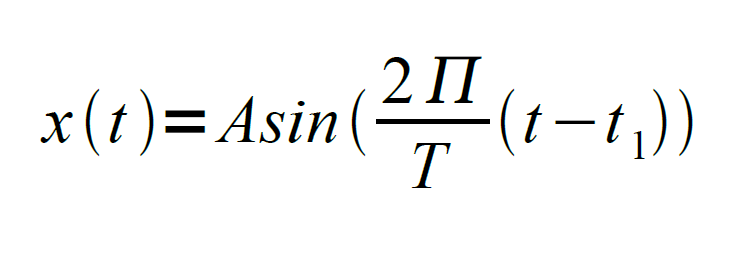
\includegraphics[width=4.3cm]{SinWzor.PNG}
 \vspace{-0.3cm}
 \label{gw}
\end{figure}

Parametry: A, T, t1, d.


\subsubsection{Przebieg}
Do generacji synału zostały podane parametry:
\addtokomafont{labelinglabel}{\sffamily}

\begin{labeling}{szj}
\item [Amplituda (A):] 2
\item [Czas trwania (t1):] 2 s
\item [Częstotliwość próbkowania (d): ] 10 Hz
\item [Okres podstawowy :] 1 s
\end{labeling}


\subsubsection{Rezultat}

Rezultaty przedstawiają zamieszczone poniżej zrzuty ekranu z programu. Wartości liczbowe oraz wykres funkcji amplitudy od czasu przedstawia \ref{Wykres dla wyników eksperymentu trzeciego}.
\begin{figure}[h!]
 \centering
 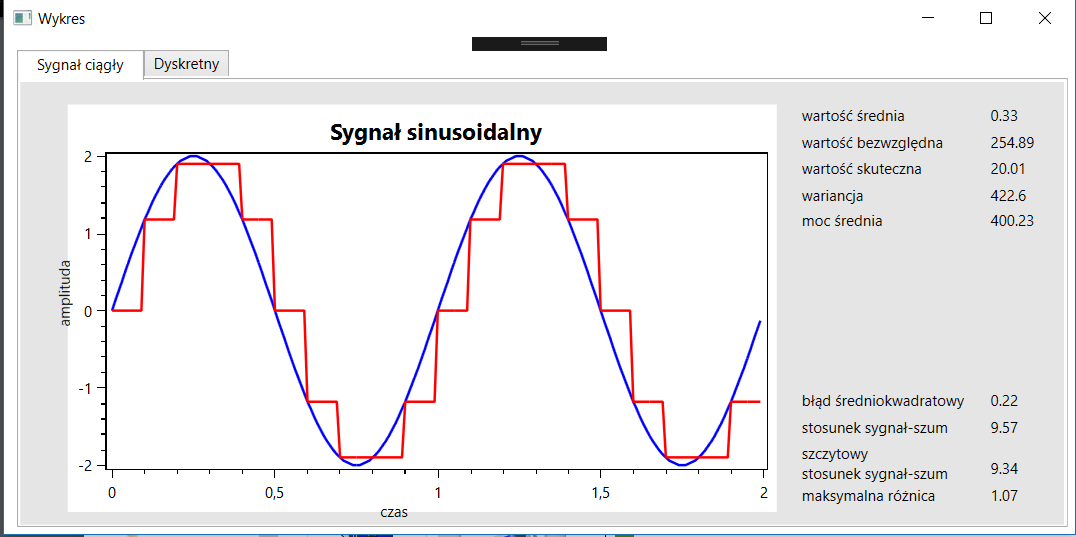
\includegraphics[width=12.3cm]{SinKwantZaokrEkstA2T2f10H2t1C.PNG}
 \vspace{-0.3cm}
 \caption{Wykres sygnału sinusoidalnego ciągły: kwantyzacja z obcięciem, ekstrapolacja zerowego rzędu}
 \label{Wykres dla wyników eksperymentu trzeciego}
\end{figure}

\newpage
Rys. \ref{Histogram dla wyników eksperymentu trzeciego} przedstawia histogram sygnału z opisanymi powyżej parametrami. 
\begin{figure}[h!]
 \centering
 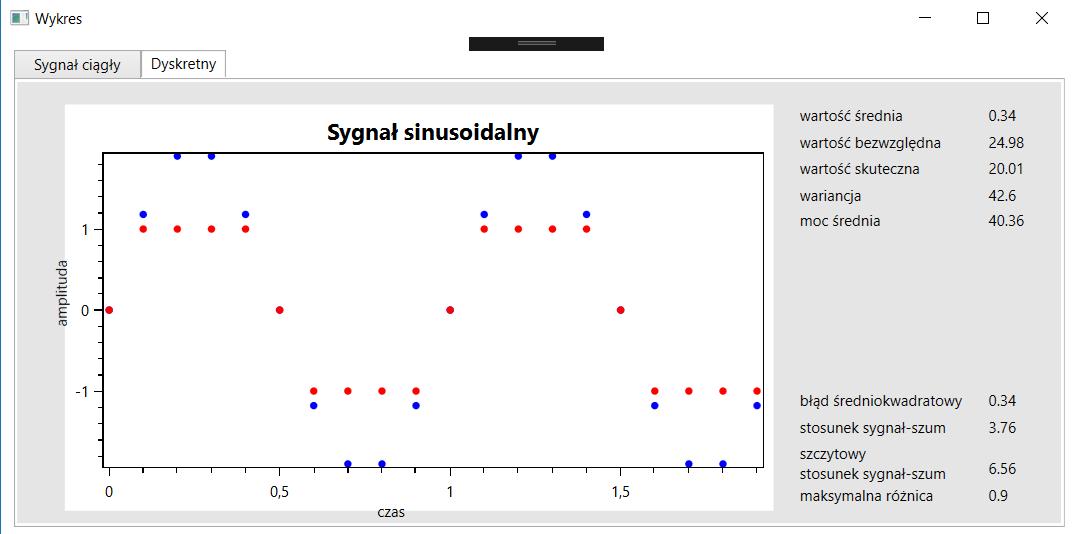
\includegraphics[width=12.3cm]{SinKwantObcrEkstA2T2f10H2t1D.PNG}
 \vspace{-0.3cm}
 \caption{Wykres sygnału sinusoidalnego dyskretny: kwantyzacja z obcięciem, ekstrapolacja zerowego rzędu}
 \label{Histogram dla wyników eksperymentu trzeciego}
\end{figure}

%%%%%%%%%%%%%%%%%%%%%%%%%%%%%%%%%%%%%%%%%%%%%%%%%%%%%%%%%%%%%%%%%%%%%%%%%%%%%%%%%%%%%%%%%%%%%%%%%%%%%%%%%%%%%%%%%
% PODROZDZIA PT. EKSPERYMENT NR4 
%%%%%%%%%%%%%%%%%%%%%%%%%%%%%%%%%%%%%%%%%%%%%%%%%%%%%%%%%%%%%%%%%%%%%%%%%%%%%%%%%%%%%%%%%%%%%%%%%%%%%%%%%%%%%%%%%

\subsection{Eksperyment nr 4}

Eksperyment nr 4 - Korelacja\\

\subsubsection{Założenia}
Do eksperymentu generujemy sygnał sinusoidalny o podanych niżej parametrach. Wejciowy sygnał analogowy zostanie zamieniony na sygnał dyskretny.
Sygnał opisuje wzór:

\begin{figure}[h!]
 \centering
 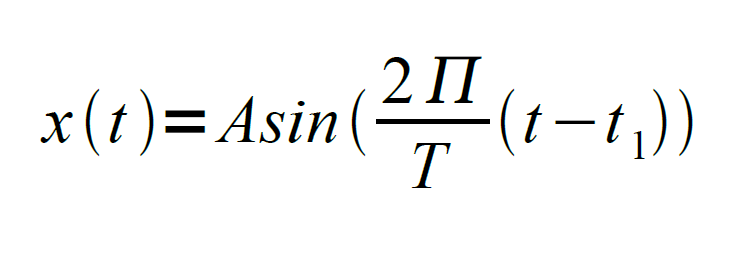
\includegraphics[width=4.3cm]{SinWzor.PNG}
 \vspace{-0.3cm}
 \label{gw}
\end{figure}
Parametry: A, T, t1, d.

W tym eksperymencie odtworzenie sygnału odbywa się porzez interpolację pierwszego rzędu, a dysktretyzacja przez kwantyzację z odcięciem. W tej metodzie wartosci sygnału pomiędzy sąsiednimi próbkami są interpolowwane za pomocą odcinków prostej.

\subsubsection{Przebieg}
Do generacji synału zostały podane parametry:
\addtokomafont{labelinglabel}{\sffamily}

\begin{labeling}{szj}
\item [Amplituda (A):] 2
\item [Czas trwania (t1):] 2 s
\item [Częstotliwość próbkowania (d): ] 10 Hz
\item [Okres podstawowy :] 1 s
\end{labeling}

\subsubsection{Rezultat}

Rezultaty przedstawiają zamieszczone poniżej zrzuty ekranu z programu. Wartości liczbowe oraz wykres funkcji amplitudy od czasu przedstawia \ref{Wykres dla wyników eksperymentu czwartego}.
\begin{figure}[h!]
 \centering
 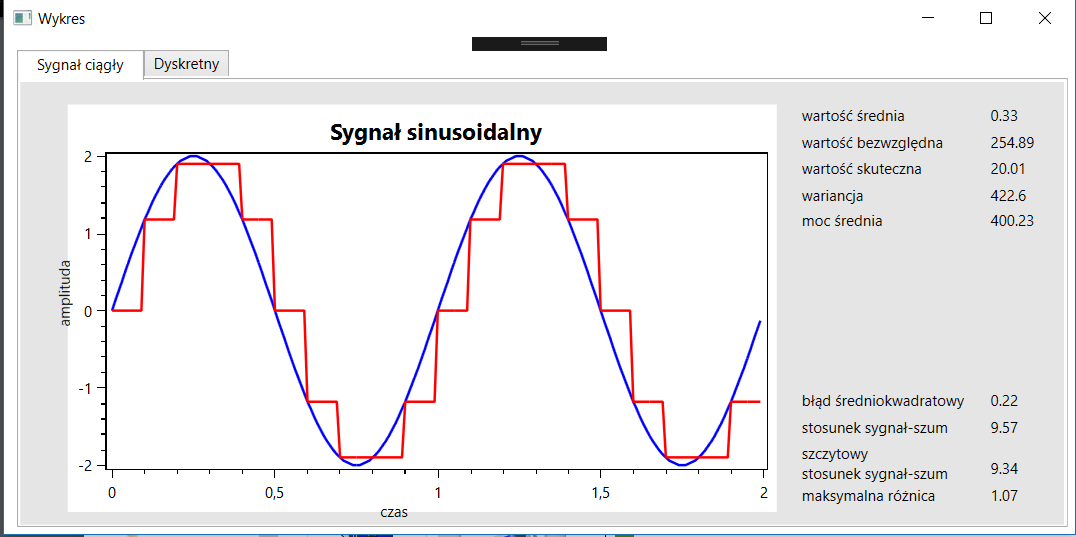
\includegraphics[width=12.3cm]{SinKwantZaokrEkstA2T2f10H2t1C.PNG}
 \vspace{-0.3cm}
 \caption{Wykres sygnału sinusoidalnego ciągły: kwantyzacja z zaokrągleniem, ekstrapolacja zerowego rzędu}
 \label{Wykres dla wyników eksperymentu czwartego}
\end{figure}

\newpage
Rys. \ref{Histogram dla wyników eksperymentu czwartego} przedstawia histogram sygnału z opisanymi powyżej parametrami. 
\begin{figure}[h!]
 \centering
 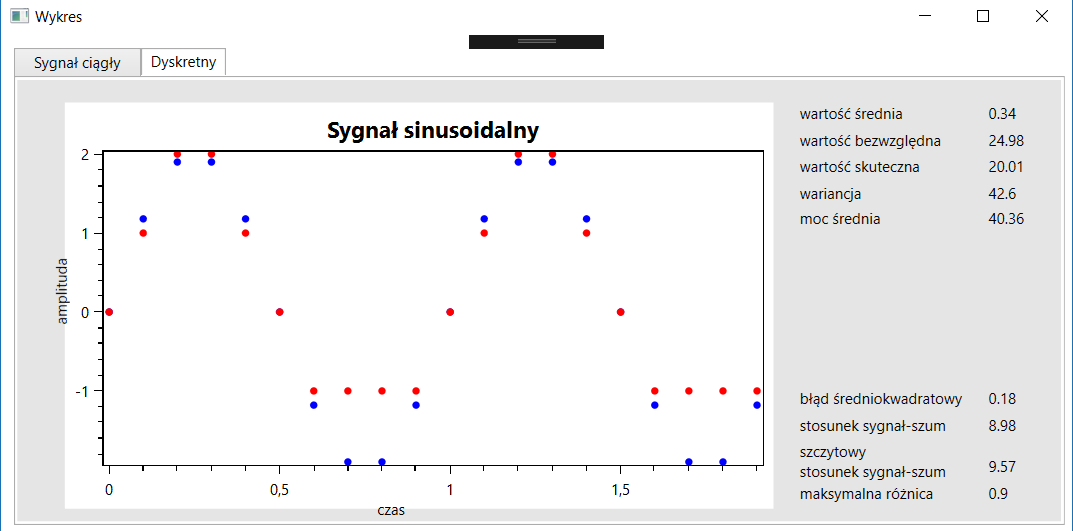
\includegraphics[width=12.3cm]{SinKwantZaokrEkstA2T2f10H2t1D.PNG}
 \vspace{-0.3cm}
 \caption{Wykres sygnału sinusoidalnego dyskretny: kwantyzacja z zaokrągleniem, ekstrapolacja zerowego rzędu}
 \label{Histogram dla wyników eksperymentu czwartego}
\end{figure}




\section{Wnioski}

Przeprowadzone eksperymenty dowodzą, że  Interpolacja pierwszego rzędu jest bardziej dokładna niż ekstrapolacja rzędu zerowego.  Dzieje się tak ponieważ między próbkami sygnał się zmienia zatem interpolowanie między kolejnymi próbkami daje lepsze odwzorowanie, niż przepisywanie tej samej wartości do czasu napotkania następnej próbki.
Aby uzyskać wyniki ekstrapolacji zbliżone do wyników ekstrapolacji należy przyjąć bardzo dużą częstotliwość próbkowania. Są znaczące róźnice w błędach odtworzenia sygnałów przez interpolację i ekstrapolację. Interpolacja jest dużo bardziej dokładna - błąd sredniokwadratowy o ok 0,2, stosunek sygnał-szum i szczytowy stosunek sygnał-szum różnią się nawet o 10 jednostek. Co ciekawe maksymalna różnica między sygnałem analogowym, a odtwarzanym sygnałem jest minimalnie większa dla interpolacji.
W przypadku kwantyzacji dużo lepiej sprawdza się kwantyzacja z zaokrągleniem. W przypadku kwantyzacji z obcięciem jeżeli próbkowaniem nie trafimy w szczyt amplitudy to maksymalna jej wartość po kwantowaniu będzie mniejsza niż ta w oryginale. Przy kwantyzacji z zaokrągleniem unikamy takiej sytuacji.
Podczas próbkowania trzeba bardzo uważać przy podawaniu częstotliwości. Jeśli podamy ją zbyt mała sygnał nie zostanie odtworzony, a czasem wręcz możemy uzyskać inny sygnał.
%%%%%%%%%%%%%%%%%%%%%%%%%%%%%%%%%%%%%%%%%%%%%%%%%%%%%%%%%%%%%%%%%%%%%%%%%%%
% PODROZDZIA PT. ZALACZNIKI
%%%%%%%%%%%%%%%%%%%%%%%%%%%%%%%%%%%%%%%%%%%%%%%%%%%%%%%%%%%%%%%%%%%%%%%%%%%
\begin{thebibliography}{0}
   \bibitem{l2short} FTIMS Politechnika Łódzka.
    \textsl{Przetwarzanie sygnałów, pojęcia podstawowe Plik}, Wikamp.
 \bibitem{l2short} FTIMS Politechnika Łódzka.
    \textsl{Zadanie 2 Generacja sygnału i szumu}, Wikamp.
\end{thebibliography}

\end{document}